\chapter{Autentificazione}

\section{Internet Security: SSL}\label{sec:isssl}
\begin{figure}[!th]
\centering
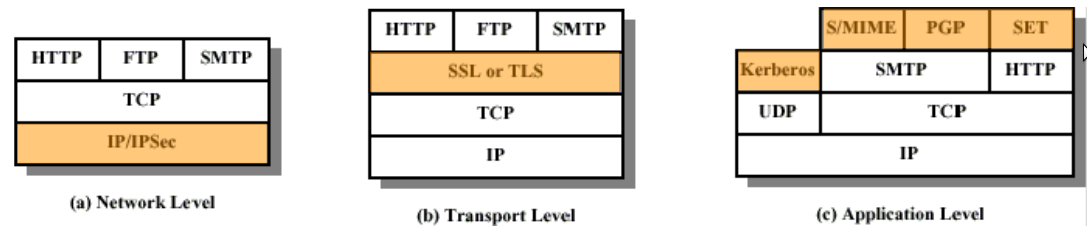
\includegraphics[scale=0.4]{images/ssl1.png}
\caption{\textit{Strati a livello OSI ove è possibile introduree SSL}.}
\label{fig:ssl1}
\end{figure}	
Nel caso della crittografia di chiave pubblica, abbiamo che, per l'utente medio,
sarebbe necessaria un'infrastruttura talmente complessa che sarebbe impossibile da
mantenere. Come si può vedere dalla figura \vref{fig:ssl1}, in quanto a livello
TCP/IP non è stato introdotto alcun criterio di sicurezza, questa è introducibile
nei seguenti livelli OSI:
\begin{description}
\item[Network Level] grazie ad \textbf{IPSec}, si inserisce la sicurezza a livello IP.
	Tuttavia, con questo metodo, anche se si può garantire la sicurezza
	per quelle applicazioni che non la richiedono, assicurando così comunicazioni protette all'interno
	di una rete potenzialmente insicura come quella pubblica, si dovrebbero
	effettuare molteplici modifiche a livello di sistema operativo. Inoltre,
	non è detto che i routers dispongano dell'architettura necessaria per
	poter gestire questi pacchetti: i router(s) infatti hanno la necessità di 
	leggere il loro contenuto, per poter instradarli successivamente: se 
	il router non riconosce quindi il pachcetto, la comunicazione con 
	un altro componente della rete non sarebbe possibile, in quanto questo
	scarterebbe tale pacchetto.
\item[Transport Level] inserendo lo strato di sicurezza tra livello applicativo
	(HTTP) e di trasporto (TCP), si ha il vantaggio di poter dialogare 
	con un nuovo livello (non più direttamente con i socket TCP) che
	garantisce in un modo immediato (simile a quello fornito dai socket)
	la sicurezza, anche se risulta necessario modificare gli applicativi,
	ma in una misura molto minore rispetto alle modifiche che è necessario
	apportare a livello di sistema operativo.
\item[Application Level] inserendo lo strato di sicurezza a questo livello, si
	ha la possibilità di garantire la sicurezza ai programmi, customizzandola
	per la particolare applicazione che la richiede, anche se questo richiede
	la riscrittura della sola applicazione, e l'adozione di molteplici 
	meccanismi di sicurezza.
\end{description}


\begin{figure}[!t]
\centering
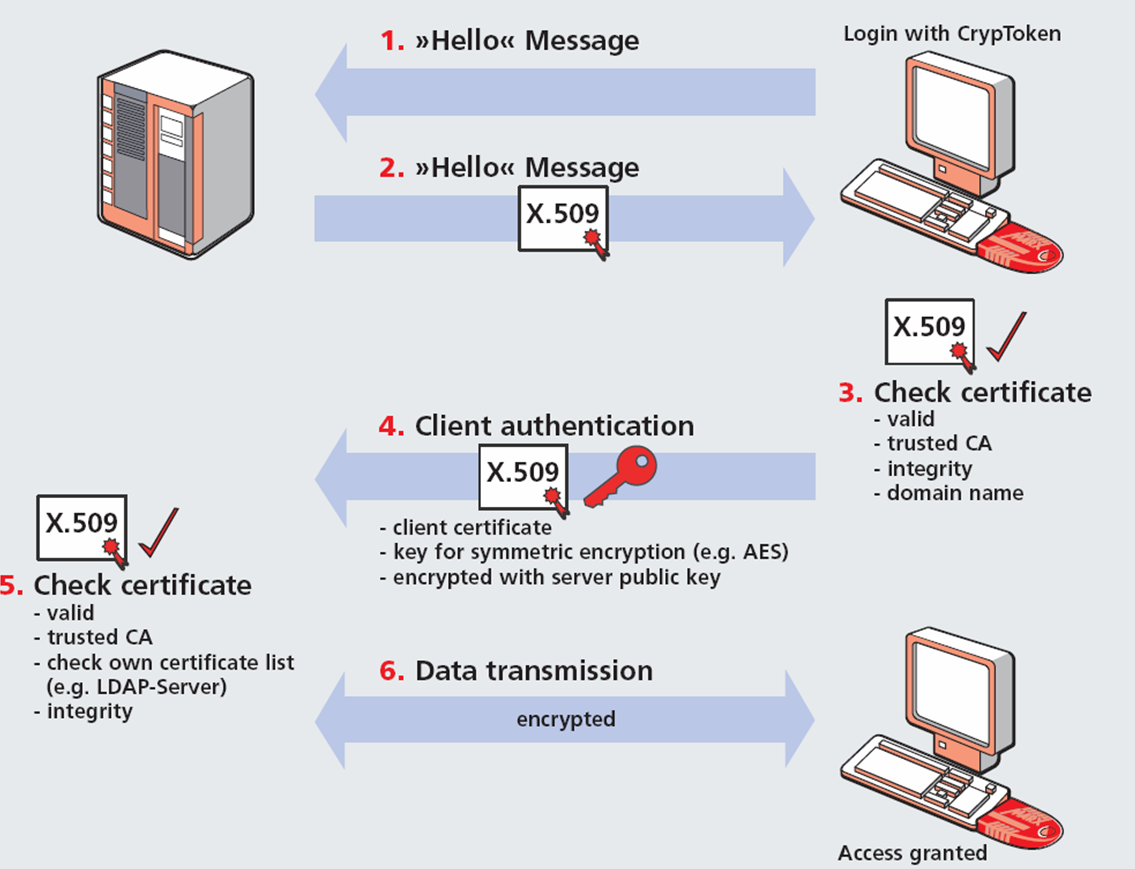
\includegraphics[scale=0.4]{images/ssl2.png}
\caption{\textit{Protocollo di instaurazione della comunicazione SSL}.}
\label{img:ssl2}
\end{figure}

Parliamo ora di come garantire sicurezza a livello di trasporto mediante SSL.
Questo nasce come protocollo di Netscape, allo scopo di garantire sicurezza
all'interno delle comunicazioni di e-commerce, che fino a quel momento non 
erano possibili in quanto Internet era nato come uno strumento di comunicazione
insicuro. Questo strumento ha quindi lo scopo di garantire \textbf{confidenzialità} 
e \textbf{autentificazione} della comunicazione in Internet. Questa è inoltre una
semplice reimplementazione di tecnologie preesistenti che vengono tuttavia
automatizzate, in modo da rendere immediata la comunicazione all'utente, senza
che questo debba preoccuparsi dei meccanismi di comunicazione che avvengono
durante una normale interazione, analoga a quella che avviene in assenza di
comunicazione sicura, dando ad esempio origine alle seguenti applicazioni che
avvengono in maniera protetta, come HTTPS, SSMTP, SFTP e SSH.


L'implementazione di SSL prevede una fase di \textbf{SSL Handshake} che è 
utilizzata per creare un canale sicuro, affidabile ed autentificato tra 
client e server, fornendo
i meccanismi di \textit{cifratura} ed \textit{autentificazione} delle chiavi,
all'interno del quale poi \textbf{SSL Record} farà viaggiare i messaggi 
incapsulandoli in blocchi cifrati ed autentificati, utilizzando la suite
fornita dallo Handshake, e fornendo i dati così ottenuti allo strato 
sottostante di TCP. Tuttavia, dobbiamo essere in grado di fornire queste garanzie
di sicurezza anche se il client ed il server, attori della comunicazione, non 
si conoscono tra loro.

Viene quindi utilizzato un protocollo descritto dall'immagine \vref{img:ssl2}:
come possiamo vedere:
\begin{enumerate}
\item Il client invia al server un messaggio di \textit{hello}
\item Il server risponde con un \textit{hello server}, fornendo il suo certificato
	(ed in rari casi richiedendo quello del client: di massima 
	questo non viene effettuato, in quanto i certificati SSL sono costosi
	da ottenere da un ente certificante). In questo caso avviene
	l'\textbf{autentificazione} del server verso il client.
\item Il client a questo punto analizza il certificato del server: a questo
	punto l'applicativo dell'utente potrebbe anche non riconoscere come
	valido il certificato ottenuto, in quanto potrebbe non essere riconosciuta
	la Root Certification Authority (che potrebbe fare riferimento allo 
	stesso server con il quale stiamo instaurando la connessione) che ha
	fornito il certificato. A questo punto l'utente potrebbe o decidere di
	rifiutare di instaurare la comunicazione, oppure decidere di accettarlo
	ritenendolo validoo grazie
	ad una conoscenza da lui posseduta ``out-of-band''.  Se il client non
	dispone di un certificato SSL, allora può essere richiesta una password
	(assieme ad un login name),
	con la quale potrà comunicare con il server senza esporre un certificato.
	Tramite questo sergreto condiviso si garantisce la \textbf{confidenzialità}
	del protocollo
\item In seguito, se la comunicazione è accettata dal server, la crittografia diventa di tipo 
	simmetrico: d'ora in poi, per rendere la comunicazione sicura, si 
	utilizzerà sempre la chiave privata fornita dal client.
\end{enumerate}

A questo punto dobbiamo distinguere la \textbf{SSL Session}, la quale è un'associazione
tra client e server a lungo termine, che si instaura con lo \textit{Handshake protocol}
e termina con l'uscita dal dominio server, dalla \textbf{SSL Connection}, che è 
scatenata da ogni interazione che avviene con il server all'interno di una stessa
sessione.

\section{Sistemi Operativi}
Gli utenti umani non sono in grado di ricordare delle chiavi (pubbliche o
private) sicure, mentre ciò potrebbe essere valido per applicazioni, come nel
caso precedente, che dialogano tra loro, e nemmeno sono in grado di effettuare
dei calcoli complicati, come quelli richiesti dagli algoritmi di crittazione e
decifrazione. 

Si rende quindi opportuno utilizzare delle regole di autentificazione, in modo
da permettere gli accessi solo ad utenti umani, o solamente alcuni di questi.
In prima istanza la coppia login-password serve proprio per garantire 
l'\textbf{autentificazione}: infatti una e-mail (come esempio di login) può 
\textbf{identificare} un solo essere umano, di cui la password associata mi garantisce 
che colui che vuole accedere, è proprio il soggetto che possiede quel dato account.
Ricordando ora i \textit{Golden Standard of security}, possiamo verificare che
l'\textbf{autentificazione} è necessaria per fornire \textbf{autorizzazione} all'accesso
di determinati utenti, tramite il quale posso anche controllare con \textbf{auditing}
le azioni che vengono compiute.

Possiamo quindi utilizzare differenti tecniche per identificare esseri umani,
chiedendo loro:
\begin{itemize}
\diam \textit{qualcosa che solo loro conoscono}: questo potrebbe essere un codice 
	PIN o una passphrase
\diam \textit{qualcosa che solo loro possiedono}: questo potrebbe essere un token,
	come ad esempio una smartcard, o comunque un oggetto che deve essere
	esibito.
\diam \textit{qualcosa che solo loro fanno}: gli esseri umani possono compiere le
	stesse azioni richieste in un modo leggermente differente tra loro
\diam \textit{qualcosa che solo loro sono}: gli esseri umani hanno delle caratteristiche
	che li distinguono tra loro, e conseguentemente possono essere utilizzate
	per effettuare una qualche forma di distinzione tra di loro.
\diam \textit{dove ti trovi}: possiamo anche garantire l'autentificazione dicendo
	che un dato utente si trova in una determinata posizione geografica.
\end{itemize}
L'unica alternativa che non necessita dello hardware aggiuntivo è la prima
opzione, in quanto le caratteristiche necessarie saranno comunque ovunque 
disponibili, mentre lo hardware per la rilevazione biometrica non è sempre
presente.


Dopo aver scelto la prima alternativa, bisogna effettuare opportuni accorgimenti:
se avviene una violazione della politica di sicurezza, questo metodo
non lascia nessuna traccia dell'abuso, e quindi non garantisce la distinzione
tra utente acceduto lecitamente e quello acceduto indebitamente. Questo
perché le password dei login associati possono essere carpite in un 
modo più meno semplificato:
\begin{itemize}
\diam Password banale od indovinata
\diam Password appuntata in un luogo molto sicuro
\diam Login spoofing
\diam Sniffing di rete (il segreto viaggia comunque in una rete)
\end{itemize}

\subsection{Metodi d'attacco delle password}
Possiamo distinguere principalmente due metodi d'attacco delle password:
\begin{description}
\item[Attacco OffLine] questo tipo d'attacco utilizza un altro sistema, all'interno
	del quale si tenta di minare l'integrità del sistema da attaccare. Per 
	effettuare questo tipo di attacco tuttavia, è necessario avere accesso
	ad una qualche informazione sulle password del sistema.
	
	A questo punto ci preoccupiamo della modalità con la quale effettuo
	il salvataggio delle password: se si memorizzassero queste all'interno
	di un file in chiaro, protetto unicamente dai metodi di controllo
	dei permessi all'interno del sistema operativo, potremo avere che 
	utenti privilegiati malintenzionati potrebbero accedervi abusando 
	delle garanzie di privacy. 
	
	Conseguentemente dobbiamo garantire in un qualche modo la \textbf{criptazione}
	delle password, utilizzando una funzone \textit{one-way hash} ottenendo
	così il fingerprint delle nostre funzioni. In questo modo si può 
	controllare la correttezza della password immessa se, per un dato utente,
	il suo fingerprint coincide con quello generato dalla password immessa.
	Tuttavi in questo modo è semplice ottenere un \textbf{dictionary attack} 
	con il quale, una volta ottenuta l'associazione tra parola e digest,
	si possa controllare se quel dato valore è presente all'interno
	di \texttt{/etc/passwd}. In questo modo, se ho trovato un match, posso
	dire di aver trovato una password che ha lo stesso hashing di quella
	inserita all'interno, riuscendo quindi ad accedere con quel login senza
	necessariamente conoscere LA password di quell'utente.
	
	A questo punto, possiamo effettuare modifiche banali sulle parole del
	dizionario, quali permutazioni, per ottenere altre possibili password
	in chiaro presenti all'interno del sistema.
	
	Questa tecnica è inoltre possibile in quanto l'attaccante è a conoscenza
	del metodo di codifica che viene utilizzato dal sistema, in quanto questa
	infomrazione è di fatti pubblica.
	
	In quanto non possiamo gestire in alcun modo il tempo che può occorrere
	tra un tentativo di attacco ed il successivo, in quanto questi avvengono
	all'interno del sistema dell'attaccante, possiamo andare ad agire sulle
	potenze di calcolo di quest'ultimo, rallentando la performance di calcolo
	delle funzioni di hash utilizzando (es. in Unix) 25 volte di seguito la 
	funzione DES. Altri modi per aumentare la sicurezza possono essere
	quelli di adottare una politica di ``salting'', o dell'ospitare i 
	codici digest in un altro file, differente dall'\texttt{/etc/password}, ovvero
	\texttt{/etc/digest}, leggibile solamente a root: in questo modo nel primo
	file, il digest della password viene sostituito da una \texttt x.
	
\item[Attacco Online] questo tipo di attacco utilizza lo stesso sistema da minare
	per poter determinare la correttezza del segreto che si vuole indovinare.
	Per limitare questo tipo di attacco si può effettuare:
	\begin{itemize}
	\diam Si può effettuare un ritardo del tempo fornito per poter effettuare
		i tentativi successivi, in modo da rallentare l'esecuzione del
		programma che effettua l'attacco.
	\diam Si può limitare il numero di tentativi errati, di modo da bloccare
		i tentativi successivi; in questo modo tuttavia si impediscono
		futuri tentativi di accessi legittimi di uno stesso login,
		rendendo quindi possibile un attacco DoS nei confronti di un utente.
	\diam Visualizzare all'atto del login l'ultimo tempo di accesso effettuato.
	\end{itemize}
	
\end{description}

Di seguito proponiamo alcune tecniche di attacco OnLine:
\begin{description}
\item[Login Spoofing] All'utente in questo caso, viene fatto credere di
	dialogare con il sistema anche se si trova di fronte ad un ``terminale
	fasullo'', il quale memorizza le sue credenziali e poi gli rifiuta 
	l'accesso al sistema che l'utente crede reale, effettuando un redirect
	a questo in un secondo momento.
	
	A questo punto, bisogna ricorrere alla nozione di \textbf{trusted path}, con
	la quale si indica un cammino, che si garantisce sicuro e quindi
	inattaccabile, tramite il quale è possibile effettuare la comunicazione
	delle password. 
	Un esempio di questo particolare trusted path all'interno dei sistemi
	Windows si ha con la combinazione di tasti \texttt{CTRL-ALT-DEL}: in questo
	modo generiamo un particolare segnale, tramite la quale possiamo 
	effettuare il lancio del login utente, in modo da essere certi di dialogare 
	con il sistema o con uno spoofer.
	Questa gestione viene effettuata ad un livello più basso rispetto a 
	quello dei driver di sistema, e per tanto non è intercettabile dagli
	applicativi che sono in esecuzione all'interno del sistema operativo.
	
	
	Tuttavia, proseguendo con un procedimento di tipo paranoico, potremmo
	arrivare ad immaginare a questo punto che sullo stesso processore
	ci possa essere presente un altro sistema operativo diverso da Windows,
	che è stato tuttavia modificato dallo spoofer in modo da apparire identico
	al precedente: per uscire da questo sarebbe sufficiente effettuare il
	reboot, a patto che lo spoofer abbia modificato anche il Master Boot
	Record. A questo punto l'unica soluzione possibile sarebbe quella di 
	riformattare il disco e reinstallare il sistema operativo, ma da un
	CD originale, e non da uno ``modificato''.
	
	A questo punto è impossibile essere in grado di stabilire una regola
	precisa per avere una garanzia in sicureza: tutto
	si basa conseguentemente su di una mera considerazione personale.
	
	Per poter premunirsi da questi attacchi, si rileva necessario il meccanismo
	di \textbf{mutua autentificazione}: mentre classicamente è solamente un utente 
	ad autenticarsi verso il sistema, che tuttavia poteva 
	essere fittizzio, ora
	un meccanismo di \textbf{challenge-response};
	il client, prima di rispondere al login, effettua una ``sfida'' con il
	sistema e, solamente se questo risponde correttamente, procederà con
	l'effettuare la procedura di login per accedervi, in un modo analogo 
	a quello che avviene tramite i certificati SSL. 
	
\item[Phishing] Oggigiorno, il login spoofing può anche essere effettuato tramite
	siti web che effettuano phishing, i quali mimano l'interfaccia del sito
	al quale l'utente effettuerà il login, esattamente come sopra, allo scopo
	di carpirne le informazioni. Questa forma di ``login spoofing'' oggi
	giorno di solito avviene tramite mail: tuttavia, grazie ai sistemi
	di DNS gratuiti quali \textbf{OpenDNS} e \texttt{8.8.8.8} di Google, oltre a 
	fornire una notevole cache (grazie alle ricerche effettuate in precedenza)
	per la conversione automatica l'indirizzo mnemonico in indirizzo IP,
	possono fornire un ottimo supporto per l'antiphishing: di fatti i siti
	che effettuano questa politica di spoofing non cambiano frequentemente,
	ed è quindi possibile rintracciarli (questi servizi lavorano inoltre
	ad un livello superiore a quello dei standard Root DNS di Internet), ed
	avvisare i visitatori del sito del tipo di contenuti in esso presenti.
	
\item[Spear-Phishing] In questo caso si intende ``lanciare un arpione per 
	pescare pesci più grossi'': il senso di questo metodo di attacco è quello
	di effettuare uno spam mirato all'interno di un azienda o comunque di
	un ambiente ben noto, con un'impostazione di contenuti molto simile
	a quella che si potrebbe ricevere all'interno di un certo ambito 
	lavorativo. Questi attacchi sono conseguentemente molto più difficili
	da identificare
\item[Keyloggers] Il \textit{keylogger} in genere è un porgramma che viene 
	installato dall'amministratore, e permette di temere una traccia di cosa 
	l'utente ha immesso all'interno del sistema da tastiera o da mouse,
	in modo da poter tracciare tutte le operazioni che lui stesso ha
	compiuto. Questi comportamenti infine sono analizzabili tramite un file
	di log finale, in modo (es.) da controllare a quali siti si effettua 
	l'accesso.
	
	Tuttavia, nell'ambito del \textbf{malaware/spyware}, questi applicativi
	possono essere installati anche a nostra insaputa, effetutando quindi
	l'inoltre delle informazioni a riguardo ad un hacker sconosciuto, che 
	verrà a conoscenza delle password che abbiamo immesso all'interno del
	nostro sistema, tramite installazione di programmi di:
	\begin{itemize}
	\item FileSharing: molti di questi programmi contengono un payload
		nascosto, ovvero un keylogger che si introduce all'interno del
		sistema
	\item Attachment alle mail di file binari, quali PDF o immagini
	\end{itemize}
	Per evitare l'installazione di questi Malaware/Sypware, si possono installare
	dei sistemi per cancellare questi programmi una volta riconosciuti.
	
	Oggigiorno, molti siti, tra cui quello della VISA, hanno modificato
	l'interfaccia utente per l'inserimento dei dati: questa presuppone
	la potenziale presenza di malaware all'interno dei sistemi, mettendo
	conseguentemente la possibilità di inserire il segreto all'interno
	del sito, non tramite utilizzo della tastiera, ma tramite una tastiera
	virtuale dalla quale selezionare i bottoni. Tuttavia, in quanto i 
	keyloggers possono anche riconoscere in quale posizione dello schermo
	è stato effettuato il click, si sarebbe in grado (ad ogni modo) di
	ricostruire la sequenza esatta dei bottoni premuti. Tuttavia, onde evitare
	questa possibilità, le sopracitate tastiere permettono la ricombinazione
	casuale dei tasti in essa contenuti.
	
	In quanto abbiamo detto che tale keylogger raccoglierà le sue informazioni
	all'interno di un file, ed in quanto certamente lo hacher sarà collegato
	in remoto con l'attaccato, potendo, quando questo si collega ad 
	internet, ottenere le informazioni contenute all'interno del file.
	A questo scopo potremmo impedire l'accesso in internet verso indirizzi
	sconosciuti o da programmi sconosciuti.
\item[Packet Sniffing] In quanto il nostro pacchetto può essere intercettato
	all'interno di una rete pubblica che, in quanto permette lo scorrere
	in chiaro delle informazioni in esso presenti, può permettere un
	attacco passivo da parte di un uditore all'interno della rete. In questo
	modo, se all'interno della rete transita un pacchetto in chiaro
	contentente una password, lo sniffer può immediatamente attaccare quell'account.
	Per evitare questo, si possono utilizzare, oltre a quelle crittografiche,
	le seguenti tecniche:
	\begin{itemize}
	\item Invece di effettuare una immissione unilaterale dell'utente,
	si può fare in modo che l'utente immetterà la sua password solamente
	dopo che il "sistema" abbia risposto correttamente alla sua sfida.
	(\textbf{Challenge-response})
	\item Invece di immettere ogni volta una stessa password, si può fare 
	in modo da utilizzare \textbf{password monouso} di modo che, se queste
	venissero intercettate, non sarebbero più utilizzabili da un attaccante.
	\end{itemize}
\end{description}

Ecco alcuni consigli che sono utili da impartire ad un amministratore di sistema:
\begin{itemize}
\diam Mai lasciare delle password di default all'interno del sistema: si avrebbe
	altrimenti una grossa vulnerabilità in quanto la password sarebbe pubblica,
	e quindi riconoscibile da tutti.
\diam Gli utenti non degono utilizzare delle password banali, perchè sarebbero
	facilmente privedibili da un attaccante, conoscendo alcuni pochi dati
	sensibili dell'utente.
\diam Ogni periodo di tempo l'amministratode del sistema dovrebbe provare a 
	minare l'integrità del sistema tramite emulazioni di possibili attacchi,
	per comprovarne la robustezza. In questo modo, l'amministratore deve 
	unicamente disabilitare gli account, finchè gli utenti corrispondenti
	non abbiano cambiato la loro password. A questo punto, è opportuno
	inserire all'interno del sistema dei vincoli tali da non far accettare
	delle password che possono risultare banali all'atto della registrazione:
	\begin{itemize}
	\item Non accettare password eccessivamente corte
	\item Anticipare i dictionary attack, non accettando talune password
	\item Accettare password con caratteri a contenuto misto, ovvero con
		elementi alfanumerici e con caratteri speciali.
	\end{itemize}
\diam Non bisogna consentire di poter effettuare dei login da remoto tramite
	programmi che chiedono un'autentificazione con la richiesta di password
	in chiaro: di solito infatti tali password viaggeranno all'interno della
	rete pubblica, e possono quindi essere soggette ad attacchi di spoofing.
\end{itemize}

Tuttavia, se è richiesto mantenere più password casuali, ciò sarebbe estremamente
difficile da memorizzare: da ciò è nata la soluzione di creare dei speciali 
software chiamati \textit{Password Manager}, i quali hanno lo scopo di memorizzare
delle password scelte dall'utente in maniera cifrata all'interno del computer.
Si può inoltre effettuare il password aging, tramite il quale ogni tanto è 
opportuno cambiare la chiave associata ad un dato login, in quanto le chiavi
private in questione potrebbero essere già state cifrate.

\section{IPSec - VPN}
Riprendiamo il tema affrontato nella Sezione \vref{sec:isssl}, tornando a chiederci
come possiamo effettuare delle comunicazioni sicure all'interno di Internet. 
Come abbiamo già notato, la sicurezza a livello \textit{network} ha il notevole 
vantaggio di rendere qualsiasi applicativo sicuro senza dover apportarvi alcun
accorgimento di sicurezza, anche se comporta di dover effettuare cambiamenti su
tutti i sistemi operativi presenti sulla rete mondiale, in quanto sia i nodi
terminali, sia quelli intermedi (vedi i routers), devono essere in grado di comunicare tramite
questo protocollo.  

\textbf{IPSec} è un insieme di protocolli\footnote{Questi sono AH (\textit{Authentication
Header}), ESP (\textit{Encapsulating Security Payload}), ed \textit{Internet Security and
Key Management Protocol}.} basati su tecniche crittografiche, allo scopo di 
fornire autentificazione e confidenzialità. Queste caratteristiche, che per ora
con IPv4 sono facoltative, saranno obbligatorie con l'introduzione di IPv6, che
verrà introdotto all'interno del protocollo di comunicazione. Una delle 
possibili applicazioni di questa tecnologia sono le \textit{Virtual Private Networks}
(VPN), e fornisce un accesso sicuro ad internet paragonabile a quello fornito a
 quello SSL. Tramite questo meccanismo, è possibile garantire sicurezza tramite
due differenti modalità di trasmissione: 
\begin{figure}[t]
\centering
\subfloat[][\emph{Rappresentazione grafica}.]
{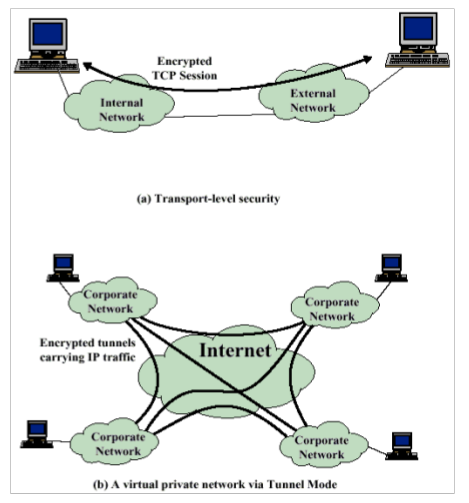
\includegraphics[scale=0.4]{images/uno.png}}\quad
\subfloat[][\emph{Incapsulamento}.]{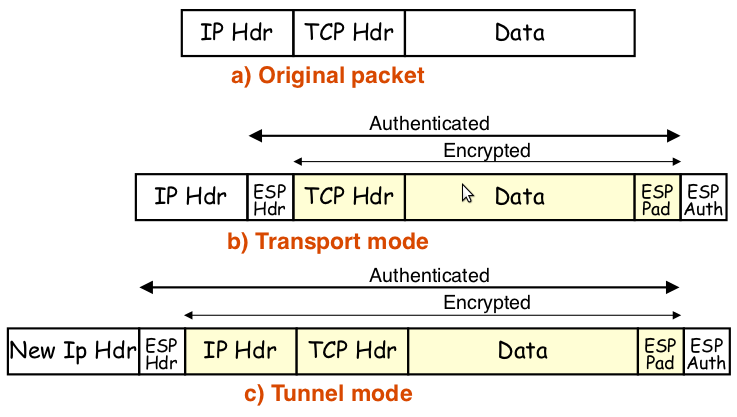
\includegraphics[scale=0.4]{images/due.png}}\quad
\caption{Rappresentazione delle differnze tra \textbf{Tunnel} e \textbf{Transport mode}.}
\end{figure}
\begin{description}
\item[Tunnel mode] fornisce una protezione dell'interno pacchetto IP, e quindi
	risulta utile per una comunicazione Gateway-Gateway come può avvenire
	nel caso delle VPN, permettendo la comunicazione sicura tra le due reti.
	In questo modo, nessuno dei suoi campi, nemmeno lo header, diventa
	leggibile all'interno della rete: è come se quindi viaggiasse all'interno
	di un tubo opaco, facendo in modo che la rete pubblica effettui l'inoltro
	del pacchetto unicamente verso il gateway di destinazione.

	Tramite la VPN di IPSec è inoltre possibile comunicare tra due parti 
	della rete aziendale connesse alla rete, che parlerà tra router a livello 
	gateway quel protocollo (emulando quindi una comunicazione PPP tra i due
	router scollegati), mantenendo invece quello IP all'interno della rete: 
	questo implica che IPSec effettua una forma di incapsulamento della 
	informazione in chiaro fornita dal semplice pacchetto IP. Questo implica 
	che gli stessi gateway devono essere in grado di tradurre i protocolli da 
	IP a IPSec e viceversa.
	
	Con questa tecnica, il gateway di destinazione ha il compito di estrarre,
	decrittare ed autentificare il pacchetto originario che è stato trasportato
	tramite incapsulamento, ed inviato dal gateway mittente. In questo modo
	viene creato un nuovo header IP, dove la comunicazione sembra avvenire
	unicamentre tramite i due gateway.
\item[Transport Mode] fornisce sicurezza a livello applicativo, e spesso è utile
	per un utilizzo end-to-end, e quindi per \texttt{TCP}: con questa modalità,
	al contrario di quella precedente, non si critta anche lo header, ma
	unicamente il payload costituito dal solo pacchetto TCP: in questo modo
	non si critta anche chi sia il mittente e la destinazione, in quanto
	queste informazioni devono essere riconoscibili proprio da chi effettua
	l'inoltro del pacchetto.
\end{description}
